% !TeX root = Bericht.tex
% !TeX spellcheck = en_US
\section{Theory}\label{sec:theorie}
In this section, the basic theoretical principles are briefly outlined to provide a better understanding of how the diode laser operates.
\subsection{ Optical Resonator}
\label{subsec:OptRes}
\begin{figure}[h]
	
	\centering
	\includegraphics[width=0.65\linewidth]{Bild Mögliche Moden}
	\caption{In this figure, it is possible to see the five first possible modes. From \autocite{BildModen}.}
	\label{fig:Moden}
\end{figure}
In an optical resonator, two mirrors are set up parallel to each other at a certain distance $L$. Due to the fact that the electric field has a node at each mirror, only waves with a wavelength $\lambda$ that is an integer inverse of the half distance between those mirrors can exist as standing waves. So we get the general relation
$$\lambda_n=\frac{2 L}{n}, $$ 
where $L$ is the length between the two mirrors. 
This behavior is shown in \autoref{fig:Moden}. It should be noted that the propagation velocity varies depending on the medium, with the refractive index given by the ratio $\eta=c/c_\mathrm{m}$, where $c$ is the speed of light in vacuum and $c_\mathrm{m}$ is the propagation speed in the medium. So with that, it is possible to find the frequencies of the standing waves between the mirrors
$$\nu_n = \frac{c_\mathrm{m}}{\lambda_n} = \frac{c}{2\eta L}\cdot n .$$
In this relation, $n$ is an Integer number, $\eta$ is the refractive index, and $L$ is the length between the mirrors. This relation can be simplified if we define the free spectral range (FSR) as $\mathrm{FSR}={c}/({2\eta\cdot L)}$. So the relation becomes $\nu=n\cdot\mathrm{FSR}$ (see~\autocite{diodenlaser}). An external factor that changes the frequency which the resonator can emit, is temperature. When heated, the entire system expands, resulting in a larger $L$. This in turn reduces $\nu$.
If the mirrors are semi-transparent, monochromatic light can be emitted. Depending on the transmittance, other frequencies can also pass through the mirror and the peaks smooth out (see~\autocite{Fabry-Perot_Interferometer_Tutorial}). This behaviour is shown in \autoref{fig:Reflexivität}. To make it clear, to get an more clear peak in the spectrum the mirrors must be more reflective.


\begin{figure}[H]
	\centering
	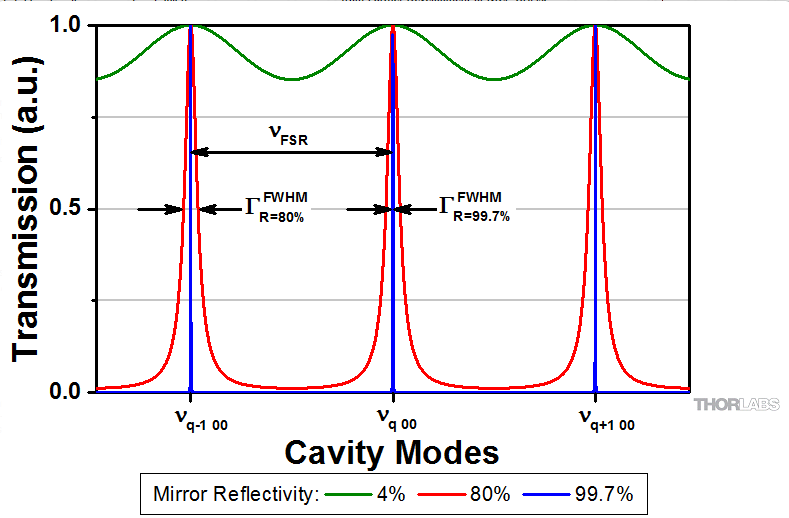
\includegraphics[clip,trim=0 0 0 2, width=0.9\linewidth]{Bild Reflektivität}
	\caption{\glqq Mode spectrum of a Fabry-Pérot interferometer for mirror reflectances of 99.7\%, 80\%, and 4\%, illustrated by a blue, red, and green curve, respectively. 99.7\% reflectance corresponds to the case for the SA200 series, which has a free spectral range of 1.5 GHz. The 4\% reflectance corresponds to a typical "fringing effect" arising from reflections between parallel surfaces on glass plates.\grqq 
		From \autocite{Fabry-Perot_Interferometer_Tutorial}.}
	\label{fig:Reflexivität}
\end{figure}


\subsection{Semiconductors}
Semiconductors, like conductors and insulators, feature a band structure composed of two key energy bands: the valence band and the conduction band. In contrast to conductors, semiconductors and insulators exhibit a gap between these bands, termed the bandgap, which is narrower in semiconductors.
The valence band houses electrons at absolute zero temperature, tightly bound to their atoms and offering minimal electrical conductivity. Above the valence band lies the conduction band, where electrons can move freely upon receiving energy, such as from an electric field or thermal excitation. Consequently, semiconductors share similarities with insulators at zero temperature.
The width of the energy gap between the valence and conduction band determines semiconductor conductivity. Insulators possess a wide gap, limiting electron mobility, while conductors feature overlapping bands enabling electron movement. Semiconductors, with their narrower gap, allow electrons to transition from the valence to the conduction band, thereby increasing conductivity under conditions like higher temperatures or through doping with impurities.
Doping involves intentionally introducing impurities into a semiconductor, such as phosphorus for n-type doping or boron for p-type doping, which alters the conductivity characteristics by introducing additional charge carriers (either electrons for n-type doping or "holes" for p-type doping) into the semiconductor crystal lattice (see~\autocite{simon2013oxford}).

\subsection{Diode Laser}\label{subsec:diode}
As already mentioned in the name, this is a diode. A diode is a semiconductor component that conducts electric current in one direction while blocking it in the opposite direction. It consists of a p-doped and an n-doped semiconductor material that are connected to each other at the so-called pn junction. In the forward direction, when positive voltage is applied to the p-doped area and negative voltage to the n-doped area, the diode allows current to flow. In the reverse direction, when the voltage is applied in the opposite polarity, the diode effectively blocks the flow of current. Diodes are used in numerous electronic circuits, including rectifiers, voltage regulators and protection circuits. 

The recombination of an electron-hole pair emits a photon. To observe this phenomenon, the semiconductor must be transparent. When n- and p-doped semiconductors come into contact with no external current, the free electrons and holes recombine and create a depletion region at the surface. Upon applying an external current, this depletion region will decrease in size, facilitating spontaneous recombination of electron-hole pairs. Eventually, the depletion region will completely vanish, allowing for the emission of a large number of photons. The current at this point is called threshold current $I_\mathrm{th}$. We expect a linear behaviour between photon power $P$ and current above $I_\mathrm{th}$ and can be represented by following function:
\begin{equation}\label{eqn:Ith}
	P(I) = \eta \left(I - I_\mathrm{th} \right).
\end{equation}
Here, the slope $\eta$ stands for the efficiency of the diode. Dividing $\eta$ with the energy one photon carries one can define the differential quantum efficiency, describing the efficiency of electron to photon conversion
$$\eta_d=\eta\frac{e\lambda}{hc},$$
where $hc/\lambda$ is the ideal energy of a photon and $e$ is the elementary charge of an electron. (see \autocite{diodenlaser}).

These behaviors not only apply to laser diodes but also characterize LEDs (light-emitting diodes). However, the phenomenon of "lasing" specifically occurs in laser diodes. In an LED, light emission results from the spontaneous recombination of electrons and holes across the semiconductor junction, producing incoherent light. In laser diodes, input current is increased until internal radiation losses become small and spontaneous emission turns into stimulated emission, creating coherent photons. Additionally, laser diodes feature an applied cavity, facilitating the production of monochromatic light, by limiting the allowed frequencies as described in \autoref{subsec:OptRes}. The schematic structure can be seen in \autoref{fig:BildLaserdiode}. It can be seen that we enclose the structure of a diode at the ends with mirrors so that the emitted photons are converted directly into monochromatic light. Most of the photons whose wavelength cannot exist in the cavity are absorbed again.

\begin{figure}[h]
	\centering
	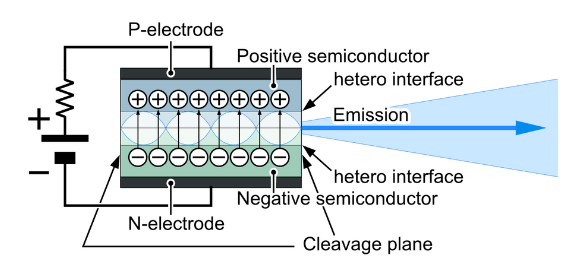
\includegraphics{BildLaserdiodeAufbau}
	\caption{The schematic layout of the laser diode can be seen in this image. The p- and n- doped semiconductors can be seen as well as the location where the cavity mirrors are attached. The direction in which the laser is emitted can also be recognised. From \autocite{WikiLaserdiode}}
	\label{fig:BildLaserdiode}
\end{figure}

\subsection{Laser modes and mode hopping}\label{subsec:modes}
As previously outlined, only specific discrete modes are emitted within a cavity. Conversely, an LED emits a Gaussian spectrum. To ascertain the modes of the laser diode, it is necessary to multiply the discrete regions within the cavity by the photon emission signal to derive the actual modes of the laser diode. The product of this behavior can be seen as an example on a 1 mm cavity in \autoref{fig:ModenLaserBild}.

\begin{figure}[H]
	\centering
	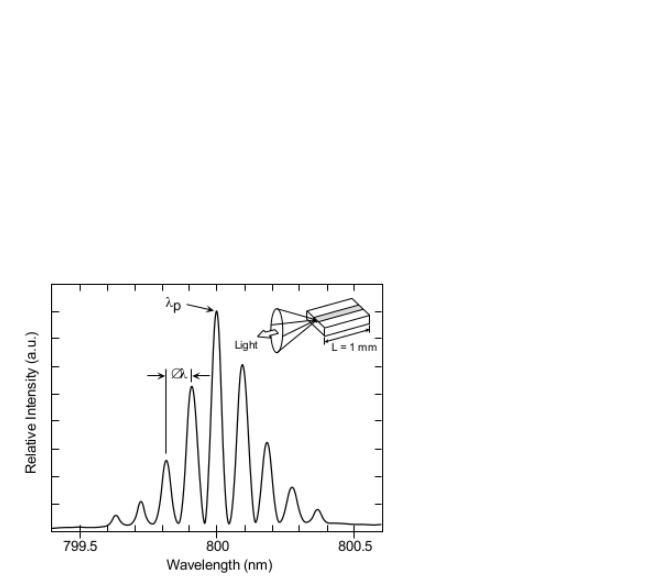
\includegraphics[width=0.8\linewidth,trim = 0 0 200 200]{Bildmoden}
	\caption{\blockcquote{Laserdiodecontrol}{Typical spectrum of an $1 \unit{mm}$ cavity length laser diode operating just above threshold. The peak wavelength of emission ($\lambda_\mathrm{P}$) is at $800 \unit{nm}$. The separation between adjacent peaks($\varnothing \lambda$) is about $0.09 \unit{nm}$.}}
	\label{fig:ModenLaserBild}
\end{figure}

If external parameters, such as the temperature of the diode, are altered, the cavity's behavior undergoes a shift, causing the spacing between frequencies to decrease and shift to the left. Consequently, the behavior of the emitted light also alters, albeit prediction of its behavior is nontrivial, since the gain profile of the diode also changes in unknown manners. Consequently, the dominant peak shifts to another, resulting in what is known as mode hopping.
%\begin{figure}[H]
%    \centering
%    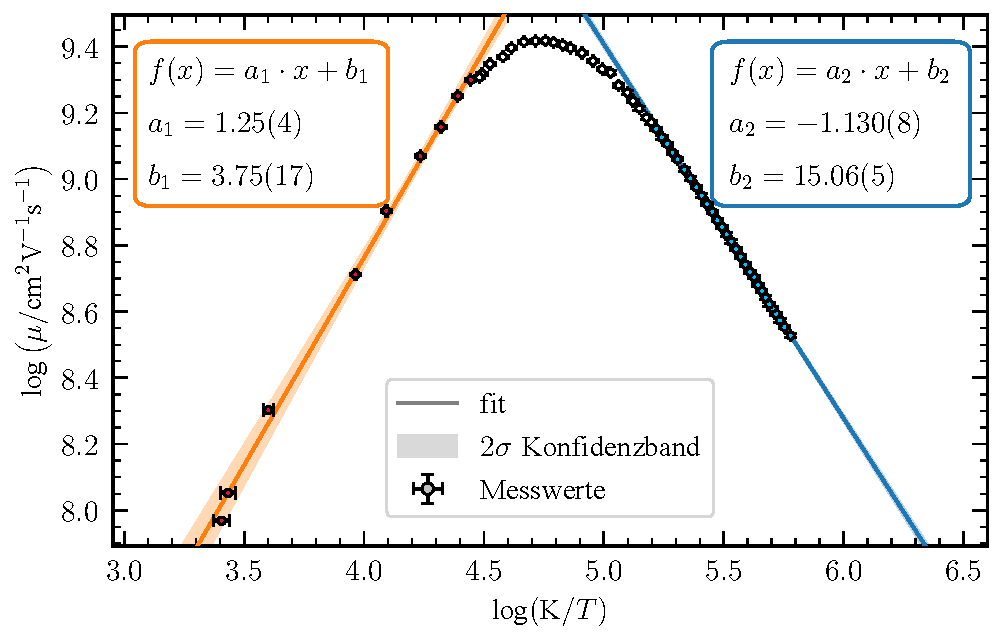
\includegraphics[width=\textwidth]{plot3.pdf}
%    \caption{}
%    \label{fig:plot3}
%\end{figure}
